% Point to the main file
\documentclass[../../Main.tex]{subfiles}

% ========== Start the document ==========
\begin{document}

\section{Section 7.4 - Expected Value}

\begin{example}
    Roullete is a game where a ball is rolled on a circular track. 
    There are 38 numbers in the track, 18 red, 18 black, 2 green. 
    If you correctly guess the number the ball lands on, you win.

    \begin{enumerate}
        \item
        {
            What is the probability that you win?

            $\boxed{\frac{1}{38}}$
        }

        \item
        {
            You play 10 times. Find the probability of winning 6 out of the 10 times.

            This is just binomial probability

            $${10 \choose 6} \; \left(\frac{1}{38}\right)^6 \left(\frac{37}{38}\right)^4 \approx \boxed{0.0000006}$$ 
        }

        \item
        {
            You play 10 times. Find the probability you never win

            $$\left(\frac{37}{37}\right)^{10} \approx \boxed{0.766}$$
        }
        \item
        {
            You play 10 times. Find the probability you win exactly once

            $${10 \choose 1} \; \left(\frac{1}{38}\right)^1 \left(\frac{37}{38}\right)^9 \approx \boxed{0.207}$$ 
        }
        
        Notice that if you graph the probabilty and wins, you get

        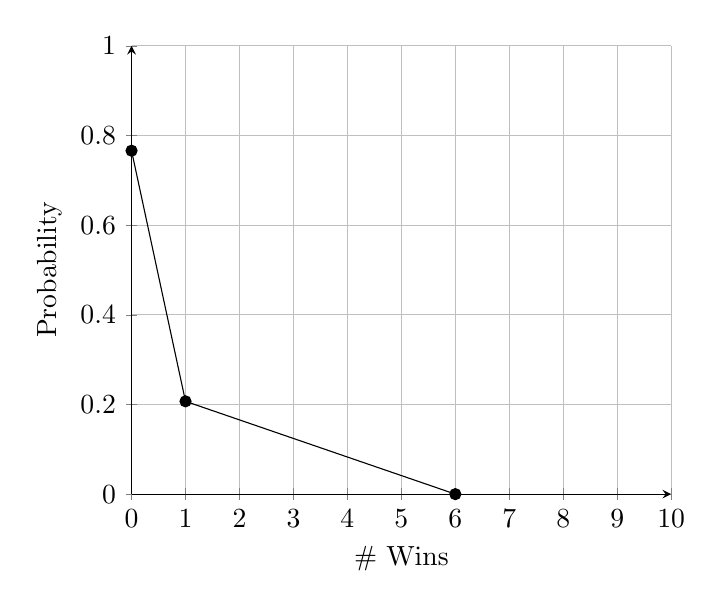
\begin{tikzpicture}
        \begin{axis}[
            xmin=0, xmax=10,
            ymin=0, ymax=1,
            xtick={0,1,2,3,4,5,6,7,8,9,10},
            ytick={0,0.2,0.4,0.6,0.8,1},
            axis lines=left,
            xlabel={\# Wins},
            ylabel={Probability},
            grid=both
        ]
        \addplot[
            mark=*,
        ] coordinates {
            (0, 0.766)
            (1, 0.207)
            (6, 0.0000006)
        };
        \end{axis}
        \end{tikzpicture}

        \item
        {
            You play 10 times. Find the probability of winning at least once

            Let's use the compliment

            \begin{align*}
                P(\text{win at least once}) &= 1 - P(\text{never win in 10 spins}) \\
                &= 1 - \left(\frac{37}{38}\right)^{10} \\
                &\approx \boxed{0.234} \\
            \end{align*}
        }
    \end{enumerate}

    In addition to guessing a number, you can also make a bet. The way it works is:

    \begin{enumerate}
        \item If you guess \# correctly, then you win $35 \times$ your bet
        \item If you guess incorrectly, then you lose your bet
    \end{enumerate}

    Now we ask, how much do we win (or lose) \textbf{on average} when making a bet?

    Assume we play a bunch of times. We bet \$1 every time

    Let's play 38 times

    Since the probability of winning is $\frac{1}{38}$, you'll probabily win 1 time and lose 37 times

    So

    \begin{align*}
        \frac{\text{total win/loss}}{\text{\# played}} &= 
            \frac{
                \overbrace{1}^{\text{\# Wins}} 
                \cdot 
                \overbrace{35}^{\text{\$ gained}} 
                + 
                \overbrace{37}^{\text{\# losses}}
                \overbrace{(-1)}^{\text{\$ lost}}
            }{\underbrace{38}_{\text{played 38 times}}} \\
        &= \boxed{-0.05} \\
    \end{align*}

    Notice that we can simplify this into

    $$
        \underbrace{\frac{1}{38}}_{\text{P(Win)}}
        \overbrace{(35)}^{\text{\$ Gained}} 
        + 
        \underbrace{\frac{37}{38}}_{\text{P(Loss)}}
        \overbrace{(-1)}^{\text{\$ Loss}}
    $$

    This is called \textbf{expected value}
\end{example}

\begin{definition}[Expected Value]
    \yellowbox{Expected Value} is the what we expect to get from a probability outcome on average.

    $$\text{EV} = \sum (\text{probability})(\text{payoff})$$

    For every case
\end{definition}

\begin{example}
    Let's go back to the roullete example

    We can also bet on red or black. If we choose correctly, we get paid the size of our bet. If we lose, we lose our bet.

    What is the expected value of betting \$1 on red?

    There are two cases.

    \begin{enumerate}
        \item We guess correctly, $P(\text{red}) = \frac{18}{38}$
        \item We guess incorrectly, $P(\text{the rest}) = \frac{20}{38}$
    \end{enumerate}

    \begin{align*}
        \text{EV} &= \sum (\text{probability})(\text{payoff}) \\
        &= P(\text{red}) \cdot (1) + P(\text{the rest}) \cdot (-1) \\
        &= \frac{20}{38} \cdot (1) + \frac{20}{38} \cdot (-1) \\
        &= \frac{-2}{38} \\
        &= \boxed{-0.05} \\
    \end{align*}

\end{example}

Let's just do one more

\begin{example}
    Toys are randomly placed in cereal boxes so that 1 out of every 6 boxes contain a toy. How many boxes \textbf{on average} must be bought to get a toy?

    There are an infinite amount of cases

    \begin{enumerate}
        \item First box contains toy, $P(1) = \frac{1}{6}$
        \item Second box contains toy, $P(2) = \frac{5}{6} \cdot \frac{1}{6}$
        \item Third box contains toy, $P(3) = \left(\frac{5}{6}\right)^2 \cdot \frac{1}{6}$
        \item You get the idea
    \end{enumerate}

    We do $\frac{5}{6}$ because all the preceding boxes DO NOT contain toys, which has a $\frac{5}{6}$ chance.

    Since the metric we are looking for is the number of boxes, the "payoff" is the number of boxes opened

    \begin{align*}
        \text{EV} &= \sum (\text{probability})(\text{payoff}) \\
        &= 
        1 \cdot \frac{1}{6} + 
        2 \cdot \frac{5}{6} \cdot \frac{1}{6} + 
        3 \cdot \left(\frac{5}{6}\right)^2 \cdot \frac{1}{6} + 
        4 \cdot \left(\frac{5}{6}\right)^3 \cdot \frac{1}{6} + \ldots \\
        &= \sum_{k = 1}^{\infty} k \cdot \left(\frac{5}{6}\right)^{k - 1} \cdot \frac{1}{6} \\
    \end{align*}

    \begin{recall}
        $$\sum_{k = 0}^{\infty} k\cdot x^k = \frac{x}{(1 - x)^2}, -1 < x < 1$$
    \end{recall}

    I'm too lazy to write out the rest so

    $$\boxed{6}$$

\end{example}

% ========== End the document ==========
\end{document}